\documentclass[dvipsnames, 9pt]{beamer}

%\documentclass[xcolor=dvipsnames, 8pt]{beamer} %
%\setbeamertemplate{navigation symbols}{}

\usetheme{SantaBarbara}

%light gray/black highlighting to be used with pause command
\colorlet{shadecolor}{gray!40}
\def\blackgray<#1>{%
  \temporal<#1>{\color{shadecolor}}{\color{black}}{\color{shadecolor}}}

\definecolor{black}{HTML}{0A0A0A}
\definecolor{red}{HTML}{e00404} 


\definecolor{blue}{HTML}{0647A8}
\definecolor{darkgreen}{HTML}{008000}

\definecolor{Asparagus}{HTML}{87A96B}

\usepackage[utf8]{inputenc}

\usepackage{tightlist}
\usepackage{tikz, tikzsettings}
\usepackage{verbatim}
\usepackage{amssymb}
\usepackage{amsmath}
\usepackage{amsfonts}
\pdfmapfile{+sansmathaccent.map} % Fix done for making the talk in ubuntu.
\usepackage{algorithmic}
\graphicspath{{./}{./figures/}{./figures/presentation/}}
\usepackage{makecell}
\usepackage{booktabs}

\usepackage{subcaption}
\usepackage[authoryear,round]{natbib}
\usepackage{color}
\usepackage{colortbl}
\usepackage{xcolor}
\usepackage{pgfplots}
\usepackage{ragged2e}
\usepackage{rxn}


\usetikzlibrary{shapes,calc,spy, calc, backgrounds,arrows, fit, decorations.pathmorphing, decorations.pathreplacing, matrix}
\usepackage{caption}
\usepackage{mpcsymbols}
\usepackage{graphicx}

\newcommand{\calert}[1]{\textcolor{blue}{#1}}

\makeatother
\setbeamertemplate{footline}
{\leavevmode%
	\hbox{%
		\begin{beamercolorbox}[wd=.3\paperwidth,ht=2.25ex,dp=1ex,center]{author
		in head/foot}%
			\usebeamerfont{author in head/foot}\insertshortauthor
		\end{beamercolorbox}%
		\begin{beamercolorbox}[wd=.6\paperwidth,ht=2.25ex,dp=1ex,center]{title
		in head/foot}%
			\usebeamerfont{title in head/foot}\insertshorttitle
		\end{beamercolorbox}%
		\begin{beamercolorbox}[wd=.1\paperwidth,ht=2.25ex,dp=1ex,center]{date in
		head/foot}%
			\insertframenumber{} / \inserttotalframenumber\hspace*{1ex}
	\end{beamercolorbox}}%
	\vskip0pt%
}

\renewcommand{\vec}{\textnormal{vec}} 
\newcommand{\stoi}{\text{\boldmath $\nu$}}


\title[Model identification]{Model identification and uncertainty prediction using deep learning}

\author[ChE230D---Dake]{Prithvi Dake}
\institute [UCSB]{Department of Chemical
  Engineering\\
    \pgfuseimage{ucsb-logo}}

\date{ChE 230D Project \\
\today}

%\AtBeginSection[]
%{
%  \begin{frame}
%    \frametitle{Outline}
%    \tableofcontents[currentsection]
%  \end{frame}}


\begin{document}

\frame{\titlepage}




\begin{frame}{Outline} 
\tableofcontents
\end{frame}

\section{Incentive for deep learning (specifically hybrid modelling)}
\begin{frame}
    \frametitle{Introduction}
    
    \begin{columns}
    {   \begin{column}{0.45\textwidth}
        \begin{block}{Motivation}
        \begin{enumerate}
        \item Interactions are difficult to model
        \item We can't use the plant for ourselves!
        \item These interactions are too expensive to investigate
        \item Some crucial intermediates are never measured (partial state measurements)
        \end{enumerate}
\end{block}
\begin{block}{Solution}
\begin{enumerate}
\item Construct a complete black-box model
\item OR use neural networks to represent diffcult-to-model portions of a first-principles model
\end{enumerate}
\end{block}
        \end{column}}
        \begin{column}{0.55\textwidth}
            \begin{figure}

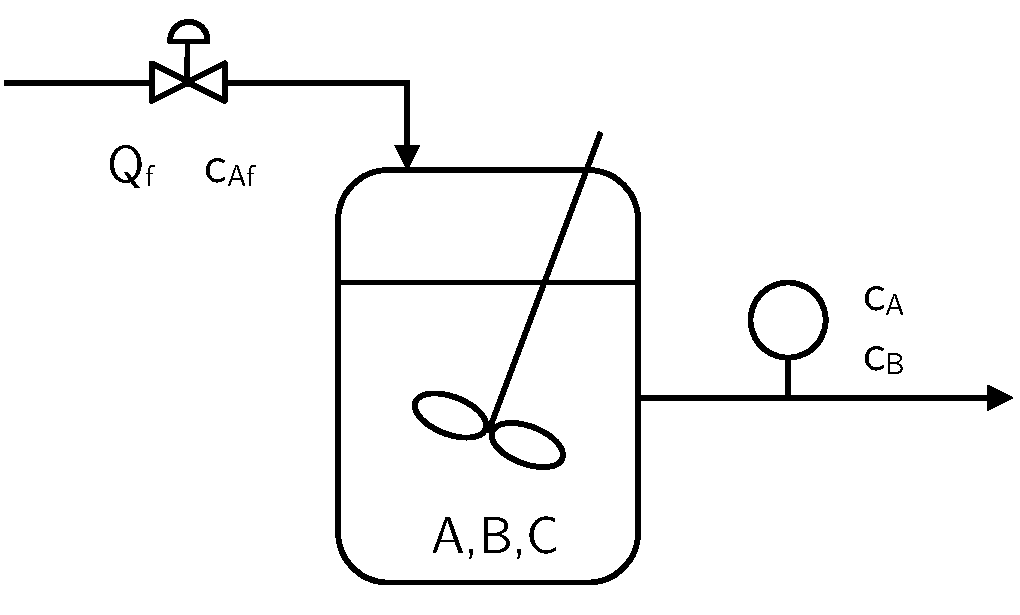
\includegraphics[width=0.8\textwidth]{process.pdf}

Don't expect data particularly useful for model building in closed-loop plants
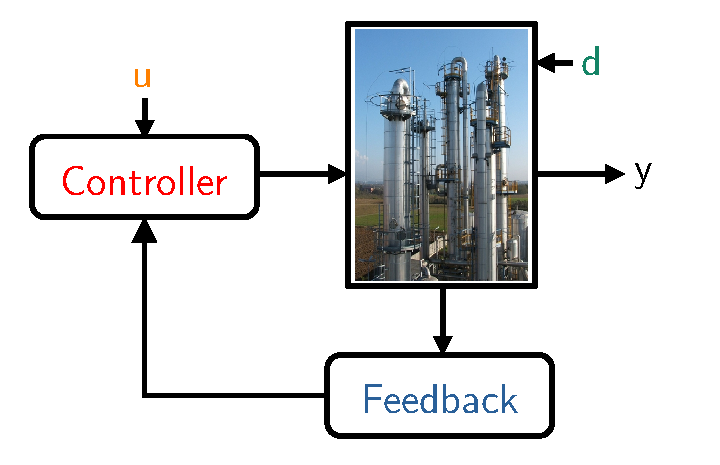
\includegraphics[width=0.8\textwidth]{control.pdf}
 \end{figure}
        \end{column}
    \end{columns}
\end{frame}



\section{Case study for partial state measurement}
\begin{frame}
    \frametitle{Sample training data}
    
    \begin{columns}
    {   \begin{column}{0.37\textwidth}
        \begin{block}{Data generating model - noise added}
\begin{align*}
\dfrac{dc_A}{dt} &= \dfrac{Q_f (c_{Af} - c_A)}{V} - r_1 \\
\dfrac{dc_B}{dt} &= \dfrac{-Q_f c_B}{V} + r_1 - 3r_2 \\
\dfrac{dc_c}{dt} &= \dfrac{-Q_f c_C}{V} + r_2 
\end{align*}
\begin{align*}
r_1 = k_1 c_A &\quad r_2 = k_2 c_B^3 - k_{-2} c_C \\
y = (c_A, c_B) &\quad u = c_{Af}
\end{align*}
\end{block}
Simulated data for the process model using PRBS signal
        \end{column}}
        \begin{column}{0.63\textwidth}
            \begin{figure}
\includegraphics[width=0.95\textwidth]{Datagen.pdf}
 \end{figure}
        \end{column}
    \end{columns}
\end{frame}


\section{Structured greybox model}
\begin{frame}
    \frametitle{Structured greybox model}
    
    \begin{columns}
    {   \begin{column}{0.57\textwidth}
        \begin{block}{Hybrid model}
\begin{align*}
\dfrac{dc_A}{dt} &= \dfrac{Q_f (c_{Af} - c_A)}{V} - \phi_1 (\mathbf{x, p}, u,\beta) \\
\dfrac{dc_B}{dt} &= \dfrac{-Q_f c_B}{V} + \phi_1 (\mathbf{x, p}, u,\beta) - 3 \phi_2 (\mathbf{x, p}, u,\beta) 
\end{align*}
\begin{align*}
y = (c_A, c_B) &\quad u = c_{Af} \\
x = [c_A, c_B]^T &\quad p = [x(t - N_p \Delta)^T, \ldots , x(t - \Delta)^T]^T 
\end{align*}
\end{block}
\begin{block}{Primer on FNNs}
\begin{align*}
\boldsymbol{\phi_i}(\cdot) &= \boldsymbol{\sigma}(\mathbf{W_i}(\cdot) + \mathbf{b_i}) \\
\beta &= (\mathbf{W_q, b_q, \ldots, W_0, b_0}) \\
\boldsymbol{\phi}(\mathbf{u}, \beta) &= \mathbf{W_q} (\phi_{q-1} \circ \ldots \circ \phi_0(\mathbf{u})) + \mathbf{b_q} \\
f \circ g &:= f(g(\cdot))
\end{align*}
\end{block}
        \end{column}}
        \begin{column}{0.4\textwidth}
            \begin{figure}
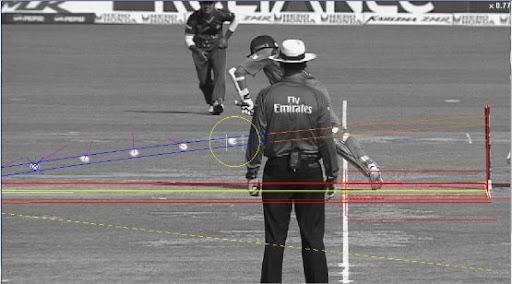
\includegraphics[width=1.\textwidth]{cricket.jpg}
\scriptsize{Reconstructing unmeasured states with history \\ Hawkeye technology in cricket \\ Famous DRS by Tendulkar on LBW \\ India won btw (World Cup 2011)!}
\newline
\begin{alertblock}{}
\begin{equation*}
L(U,Y,\beta) = \sum_{i=1}^{N_tr} \sum_{k=0}^{N_t} |y_i(k) - \hat{y}_i (k)|^2
\end{equation*}
\begin{enumerate}
\scriptsize
\item Custom integrator like RK4
\item Take care to simultaneously update the past vector \textbf{p}
\item $\dfrac{\partial L}{\partial \beta}$ use autodifferentiation libraries
\item Eg. Pytorch, TensorFlow or JAX
\end{enumerate}
\end{alertblock}

 \end{figure}
        \end{column}
    \end{columns}
\end{frame}






\begin{frame}{Resources}
\begin{figure}[H]
\centering

\includegraphics[width=0.1\textwidth]{jax_logo.png}
\end{figure}
\end{frame}
\end{document}
